% !TEX encoding = UTF-8
% !TEX TS-program = pdflatex
% !TEX root = ../tesi.tex

%**************************************************************
\chapter{Metodi di Machine Learning}
\label{cap:ML}
%**************************************************************
\intro{Questo capitolo illustrerà i metodi di \emph{Machine Learning} che sono stati utilizzati per la predizione degli esiti delle partite di calcio della Seria A italiana della stagione 2021/2022. Purtroppo, non è stato possibile applicare metodi di \emph{Machine learning} che corrispondessero al modello \emph{Bradley-Terry} perché, nonostante esistano metodi in \emph{Machine learning} che forniscono modelli basati sul modello \emph{Bradley-Terry}, essi non sono in grado di gestire l'esito del pareggio ma solo un esito binario. Ne consegue che tali metodi non sono adatti per contesti come il calcio ma ad altri tipi di sport dove il pareggio non è previsto come il \emph{baseball}. I metodi di \emph{Machine learning} considerati sono: il K-Nearest-Neighbors (KNN), la Support Vector Machine (SVM), gli alberi di decisione per la classificazione, la Random Forests e in fine l'Adaboost.
}
\section{Componenti essenziali}
In questa sezione vengono definite alcune misure e tecniche che sono necessarie per il funzionamento dei metodi di \emph{Machine Learning} applicati.
\subsection{Distanza di Minkowski}
La \textit{\cite{minkdist}} è una misura utilizzata per la valutazione della distanza ovvero, nel nostro contesto della somiglianza tra due punti in spazio di \textit{n}-dimensioni. La distanza di Minkowski di ordine \emph{d} tra due punti A = (a$_1$,...a$_n$) e B = (b$_1$,...b$_n$) vale
\begin{center}
	$Dist(A,B) =  \left(\sum_{i = 1}^{n}|a_i-b_i|^d\right)^{1/d} $
\end{center}

Si sottolinea che quando l'ordine d = 1, la distanza utilizzata è la \textit{\cite{manhattan}} ovvero la distanza tra due punti è la somma del valore assoluto delle differenze delle loro coordinate. Quando l'ordine d = 2 è applicata la \textit{\cite{euclidea}} dove la distanza tra due punti è la lunghezza del segmento con agli estremi i due punti d'interesse.
Tale misura sarà utilizzata nel metodo K-Nearest-Neighbors (KNN).
\subsection{Funzione kernel}
Nel contesto dell'apprendimento automatico, la \textit{\cite{kernel}} permette di trasformare uno spazio di input non linearmente separabile in uno nuovo spazio delle istanze di input detto \emph{feature space} di dimensione superiore rispetto a quello originale tale da diventare linearmente separabile. Per spazio linearmente separabile si intende che esiste un iperpiano in grado di separare correttamente i dati in due gruppi distinti. Perciò aumentando la dimensionalità dello spazio d'interesse è possibile trovare la dimensione opportuna che permetta di separare linearmente i dati. Tale applicazione è chiamata kernel trick. Perciò, una funzione kernel è una funzione \emph{K} che per ogni \emph{x}, \emph{y} $\in \chi$ dove $\chi$ è lo spazio di input di dimensione \emph{n}, vale 
\begin{center}
	$K(x,y) =  \langle\psi(x),\psi(y)\rangle $.
\end{center}
Dove $\psi$ è la funzione che mappa i punti di uno spazio di dimensione \emph{n} in uno spazio di dimensione \emph{m} con \emph{m>n}, invece, $\langle . \rangle$ indica il prodotto scalare.\\
Nelle nostre predizioni saranno usati questi kernel:
\begin{itemize}
	\item Linear kernel: è la funzione precedentemente definita.
	\item Polynomial kernel: $K(x,y) =  \left(1 + \sum_{i = 1}^{p}x_iy_i\right)^{d} $ dove \emph{p} è il numero di istanze di input presenti in $\chi$ mentre \emph{d} la dimensione del spazio (l'ordine).
	\item Gaussian Radial Basis kernel (RBF): $K(x,y) = exp(-\gamma||x-y||^2) $ con $\gamma=\frac{1}{2\sigma^2}$ mentre $\sigma$ è un paramento libero. 
\end{itemize}
La funzione kernel sarà utilizza nella Support Vector Machine (SVM).

\subsection{Bootstrap}
In statistica e nell'apprendimento automatico, per \textit{\cite{bootstrap}} si intende una tecnica di ricampionamento per la generazione di un insieme di campioni di \emph{m} osservazioni contenute da un dataset di dimensione \emph{n}. Ogni estrazione è casuale e con rimpiazzo, cioè un’osservazione può essere presente in più campioni. Tale tecnica è utilizzata per produrre un insieme di campioni che siano il più possibile rappresentativi e indipendenti tra di loro.\\

Nella Figura \ref{fig:bootstrap} viene mostrato un esempio della procedura di \emph{Bootstrap}

\begin{figure}[]
	\begin{center}
		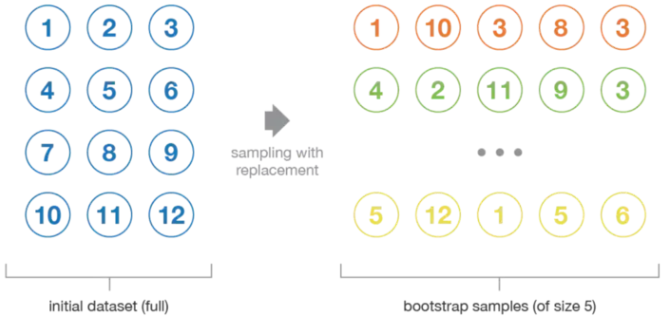
\includegraphics[scale=0.60]{bootstrap1.png}
		\caption{Esempio grafico della procedura di \emph{Bootstrap}.
		} 
		Source: \url{https://blog.paperspace.com/bagging-ensemble-methods/}\label{fig:bootstrap}
	\end{center}
\end{figure}

\subsection{Bagging}
Il Bagging \textit{\cite{breiman1996bagging}} detto anche \emph{Bootstrap Aggregation Approch}, è una tecnica \emph{ensemble learning} di tipo parallelo che dalla mediazione di più predizioni fatte da un insieme di classificatori deboli ottiene un'unica predizione finale. È di tipo parallelo perché va a sfruttare l'indipendenza dei classificatori. La procedura applicata è la seguente:
\begin{itemize}
	\item Creazione di k campioni utilizzando la tecnica di \emph{Bootstrap}.
	\item Per ogni campione viene allenato un classificatore.
	\item Viene prodotta una predizione per ogni classificatore allenato.
	\item Le predizioni ottenute vengono mediate ottenendo un predizione finale.
\end{itemize} 
Una tecnica per mediare è ad esempio, il \emph{voting} dove la classe più predetta sarà il risultato dalla predizione finale.Inoltre, si utilizza il \emph{Bootstrap} per rendere i classificatori indipendenti tra di loro.
Perciò l'obbiettivo del \emph{Bagging} è quello di creare un classificatore modello di gestire un'elevata varianza dei dati in modo efficiente grazie al parallelismo.\\
Nella Figura \ref{fig:bagging} viene illustrato graficamente la procedura di \emph{Bagging}

\begin{figure}[]
	\begin{center}
		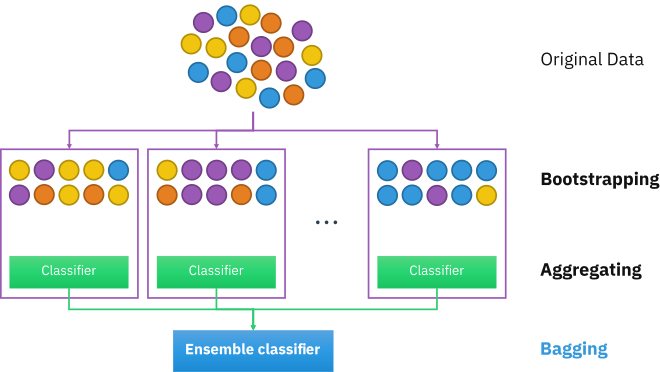
\includegraphics[scale=0.50]{Ensemble_Bagging.png}
		\caption{Esempio grafico della procedura di \emph{Bagging}.
		} 
		Source: \url{https://www.analyticsvidhya.com/blog/2020/02/what-is-bootstrap-sampling-in-statistics-and-machine-learning/}\label{fig:bagging}
	\end{center}
\end{figure}

\subsection{Boosting}
Il Boosting \textit{\cite{freund1996experiments}} è una tecnica \emph{ensemble learning} di tipo sequenziale che sfrutta la dipendenza tra i classificatori usati. Sostanzialmente l'algoritmo inizialmente allena un classificatore debole con tutto il \emph{dataset} a disposizione. Successivamente per raffinare la predizione vengono allenati in sequenza nuovi classificatori che apprendono da tutto ciò che è stato appreso dal classificatore precedente e dal l'intero \emph{dataset}.\\
La procedura completa è la seguente:
\begin{itemize}
	\item Viene utilizzato l'intero \emph{dataset} per allenare un classificatore debole.
	\item Vengono ripesati gli esempi di \emph{training} dando un peso maggiore a quei esempi a cui che è stata sbagliata la classificazione, viceversa per gli esempi classificati correttamente.
	\item Ripetere per n volte i passi precedenti con un nuovo classificatore con i pesi aggiornati.
	\item Combinare tutte le ipotesi semplici in un unico classificatore accurato per ottenerne il risultato finale.
\end{itemize}
Perciò con l'aggiornamento dei pesi si presuppone che i classificatori successivi non andranno a commettere gli stessi errori dei classificatori precedenti.\\
L'obbiettivo del\emph{Boosting} è concentrare i propri sforzi nel creare un classificatore adatto a gestire un'elevata distorsione anziché un'elevata varianza dei dati. Infatti, partendo da un classificatore debole e migliorandolo in modo sequenziale, si consente ai classificatori successivi di imparare dagli errori precedentemente commessi, riducendo la distorsione dei dati. Inoltre, il \emph{Boosting} è la resistenza agli effetti dell'\emph{overfitting}.
Purtroppo, il \emph{Boosting} risulta molto sensibile ai valori anomali e inoltre, dato che le operazioni di addestramento di ogni classificatore avvengo in modo sequenziale non sarà possibile utilizzare il parallelismo per risparmiare tempo di calcolo.\\
Nella Figura \ref{fig:boosting} viene illustrato graficamente la procedura di \emph{Boosting}

\begin{figure}[]
	\begin{center}
		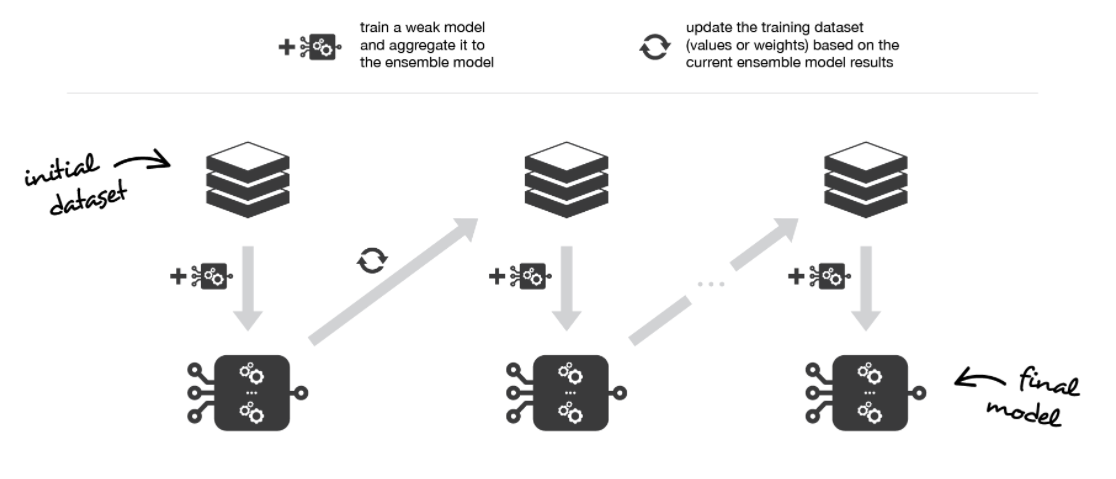
\includegraphics[scale=0.60]{boosting.png}
		\caption{Esempio grafico della procedura di \emph{Boosting}.
		} 
		Source: \url{https://www.section.io/engineering-education/boosting-algorithms-python/}\label{fig:boosting}
	\end{center}
\end{figure}
